% Chapter Template

\chapter{Experiments for Parameterized Reduced Order Models} 
\label{Chapter5}

The previous examples showed the feasibility to use the POD-DEIM approach on marine ecosystem models with a fixed 
set of parameters. In \cite{PODDeimapplication}, the authors propose to use the POD-DEIM approach for parameter studies of dynamical 
systems. In this case, it means to simulate the full-order model for multiple parameter sets and
use all the snapshots to create a reduced-order model. To investigate this the N-Model with one tracer is used again, but this time with different parameter sets. Since the parameter space is quite large, 
Latin Hypercube sampling, as proposed in \cite{ROM_book2}, is used to generate ten samples (cf. Table \ref{Chapter5:table_lhc_sample}) within the bounds
that are given in Table 2 in \cite{metos3dsimpack}. In Chapter \ref{Chapter4}, the amount of snapshots for the smallest setup of viable ROM was $36 \cdot 1000= 36000$ snapshots.
Thus, for every parameter sample 36000 snapshots are used. Since a SVD must be computed of the whole 
snapshot matrix, there exist a soft upper bound for the number of snapshots, and thus, for the number of parameter samples.
The combined snapshot matrices are
\begin{equation*}
 S =[Y_1|\dots|Y_9], \quad S_q = [Q_1|\dots|Q_9],
\end{equation*}
where $Y_i$ and $Q_i$ are the snapshot matrices of the solution corresponding to the Latin Hypercube sample $i$.
These are in total 360000 snapshots, thus, the matrices $S$ and $S_q$ have the dimension $52749 \times 360000$.
The singular values of this SVD are visible in Figure \ref{fig:singularvalues_10_lhc}. They decrease much slower than the ones in Figure \ref{fig:comparison_differnt_singuarvalues} from the N-Model.
\begin{figure}[ht]
\centering
  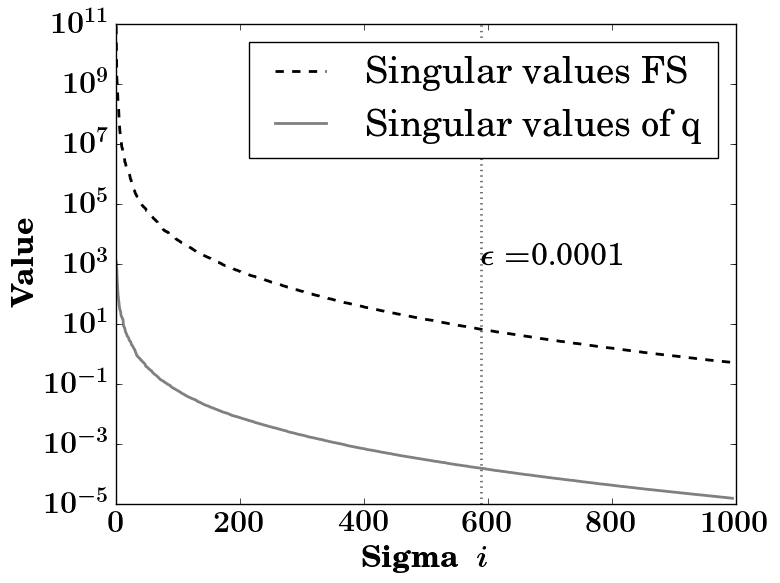
\includegraphics[width=0.7\textwidth]{singularvalues_10_lhc_1000.png}
  \caption{Distribution of singular values of $S$ and $S_q$.}
  \label{fig:singularvalues_10_lhc}
\end{figure}
The singular values of the full system matrix decent only to a value near $10^0$, this is much higher than the previously showed singular values.
The approximated error bound of a ROM, created out of the corresponding left singular vectors, is tremendously high, in an order of $10^4$.
It was not possible to create a ROM that generates a solution that is close to the original for any of the parameter sets listed in Table \ref{Chapter5:table_lhc_sample}, with which the model was created. The relative 
error is always over 1 and it is oscillating a lot in the course of 3000 model years, cf. Figure \ref{fig:error_norm_lhc_0}. With a new parameter set that was not used to create the model, for example 
$1.5 \cdot u_r = u_r + 50\% = \{0.03,3.,0.75,45.,1.287\}$, the result is similar. The ROM, created out of multiple solution trajectories, is very inaccurate, cf. Figure \ref{fig:error_norm_+50}.
Thus, the approach to create one ROM out of multiple trajectories seems not to lead to an accurate and useful one. One possible explanation for this is the diversity of the solutions that the FOM generates for different parameter sets.
Together, they can not be well approximated within the same low dimensional subspace. Therefore, the subspace, generated by the POD method, is only a poor approximation. 

Another idea is to create multiple ROMs for multiple parameter sets. And then for a new parameter set use the ROM that was created with the parameter set that is the closest to the new one. 
This approach should be possible if a ROM can produce an acceptable solution also for a set of parameters 
that is different from the parameter set the ROM has been created with.
To try this out, four parameter sets are taken. The parameter sets are deviations from the reference parameter set $u_r + x\%$ with $x\in \{5,10,20,50\}$.
Using the ROM $36\_3000P300D300$, from Chapter \ref{Chapter4_N}, which was create with the parameter set $u_r$, simulation are made. 
The relative error between these spin-ups and the corresponding original solution of the FOM is shown in Figure \ref{fig:error_norm_one_base_+50}. In the figure it is visible that the further away the parameter set from $u_r$ is, the larger becomes the relative error of the solution of the ROM to the original solution of the FOM. 
All spin-ups show a decrease of the error in the first half of the 1500 model years and an increase in the second half of the 3000 model years. The further away the parameter set is, the earlier the relative error begins to increase. 
The relative error is in the order of $10^{-1}$, thus, the solution that the ROM generates for a different set of parameters, seems to be not usable.  
The dashed lines with the left arrow show the relative error between the two FOM spin-ups. One spin-up was executed with parameter set $u_r$ and the other spin-up was run with one of the deviations $u_r + x\%$. Plotted in order 5, 10, 20, 50 from bottom to top. Compared to corresponding relative error of the FOM, the solutions of the ROMs are most of the time less accurate. And it seems that carrying out a ROM simulation with a different set of parameters does not lead to a significant change in the solution. The change is larger, the further away the set of parameters is, but then, there is a stronger divergence after around 1000 model years.

\begin{figure}[ht]
\centering
  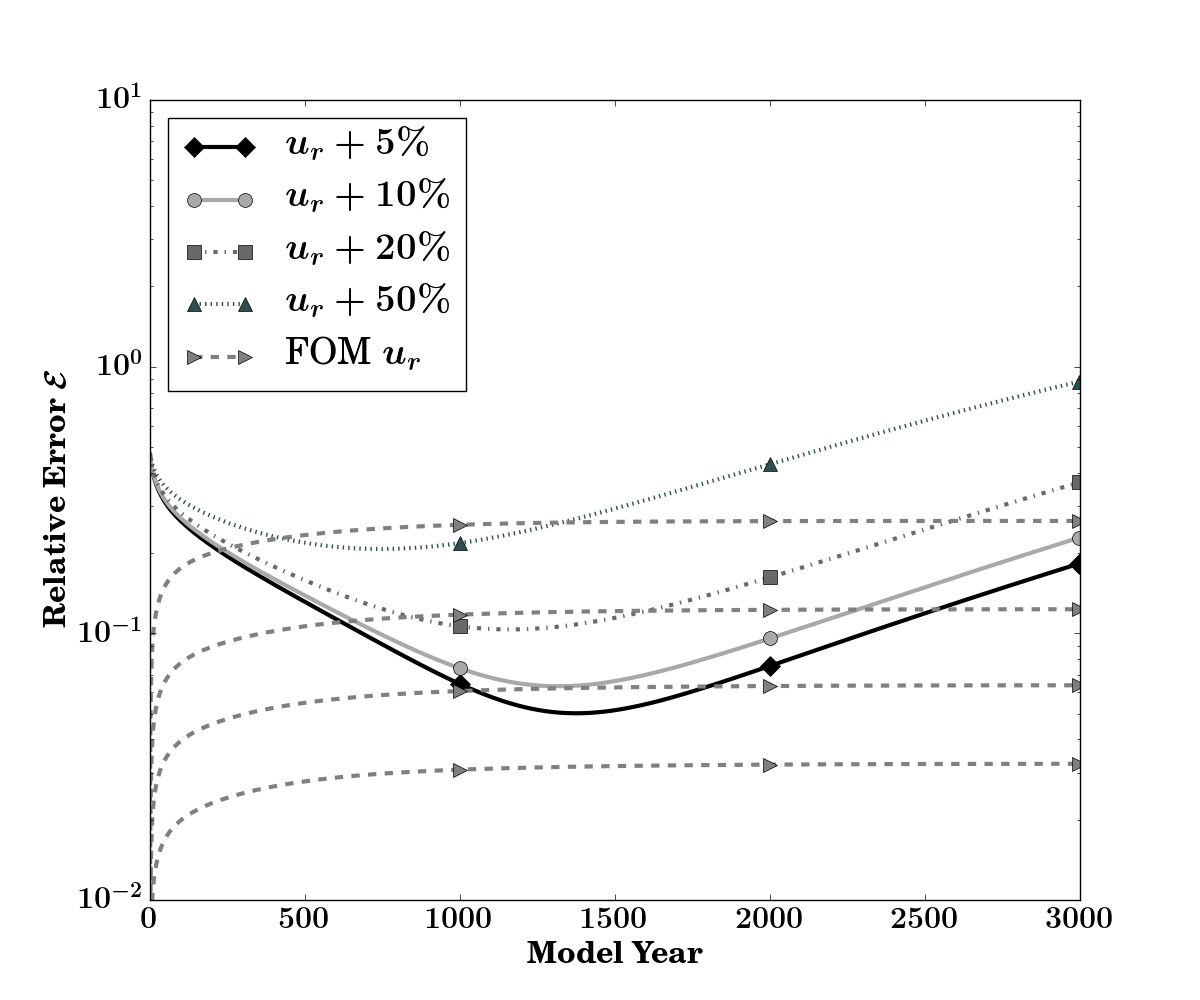
\includegraphics[width=0.9\textwidth]{error_norm_one_base_+50.png}
  \caption[The relative error between the ROM $36\_3000P300D300$ and the FOM for different sets of parameters.]{The relative error between the ROM $36\_3000P300D300$ and the FOM for different parameter sets $u_r + x\%$, where $x\in \{5, 10, 20, 50\}$. The dashed lines with the left arrow show the relative error between 
  the FOM spin-up with parameter set $u_r$ and one of the deviations $u_r + x\%$. Plotted in order 5,10,20,50 from bottom to top.}
  \label{fig:error_norm_one_base_+50}
\end{figure}

In Figure \ref{fig:error_norm_one_base_+50_FOM_+0}, the relative error between the ROMs spin-ups for the parameter sets $u_r + x\%$ with $x \in  \{5,10,20,50\}$ and the FOM solution of $u_r$ is visible. The error is
large, which means that the spin-ups of the ROM are not close to the original solution of the FOM using the parameter set $u_r$. Thus, the ROM results in a completely different solution if it is executed with a different parameter sample than it was created with and they start to diverge early. 

In conclusion, executing a ROM with a different set of parameter than it was created with does not lead to a usable solution. Thus, the idea of creating multiple ROMs and using them for parameter studies seems not to be feasible. Overall, it has not been possible to find a ROM or multiple ROMs that can be used for new sets of parameters and resulting in an acceptable solution.
\begin{figure}[ht]
\centering
  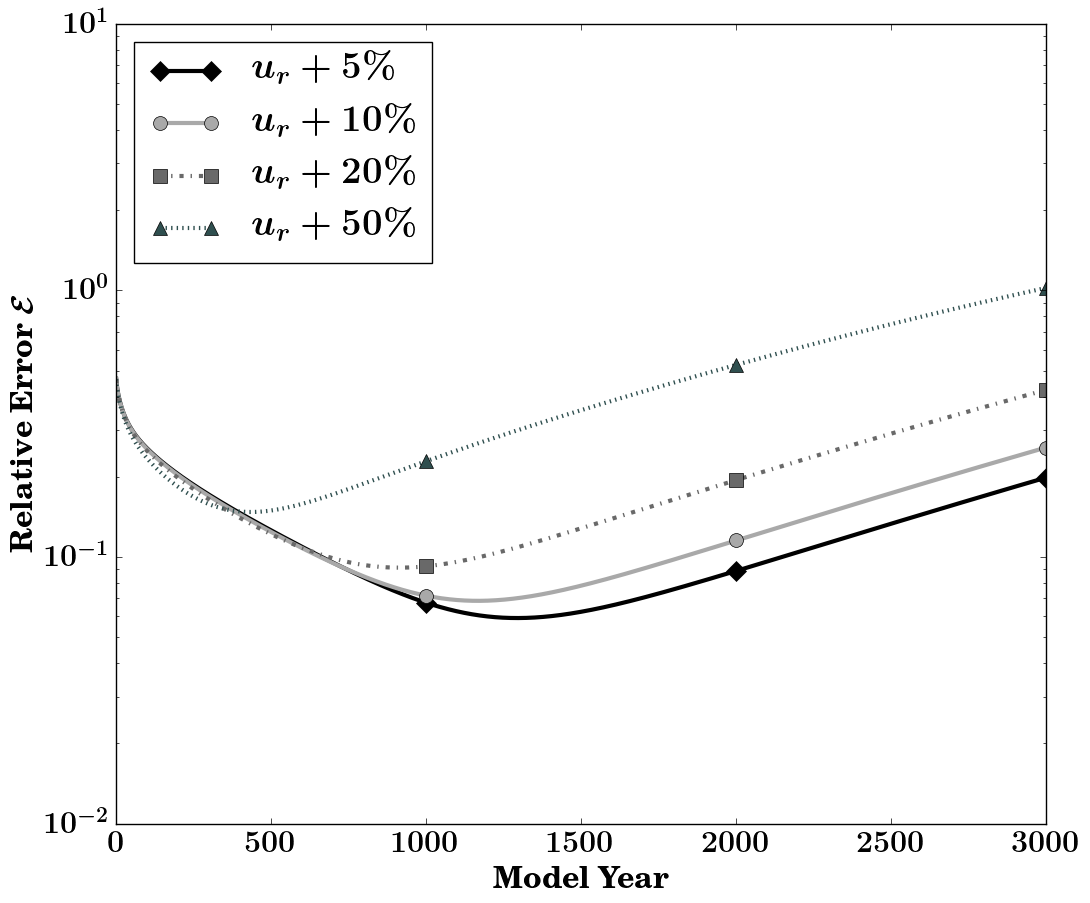
\includegraphics[width=0.9\textwidth]{error_norm_one_base_+50_FOM_+0.png}
  \caption[The relative error between the ROM $36\_3000P300D300$ and the FOM solution of $u_r$.]{The relative error between the ROM $36\_3000P300D300$ for the parameter sets $u_r + x\%$  and the FOM solution of $u_r$, where $x\in \{5,10,20,50\}$.}
  \label{fig:error_norm_one_base_+50_FOM_+0}
\end{figure}
